\chapter{Alejandro Hernández Cano}

\section{Sobre mi}
Me llamo Alejandro y estoy cursando el propedeutico de Ciencias de la
Computacion en la Facultad de Ciencias de la UNAM.

\begin{figure}[h]
  \centering
  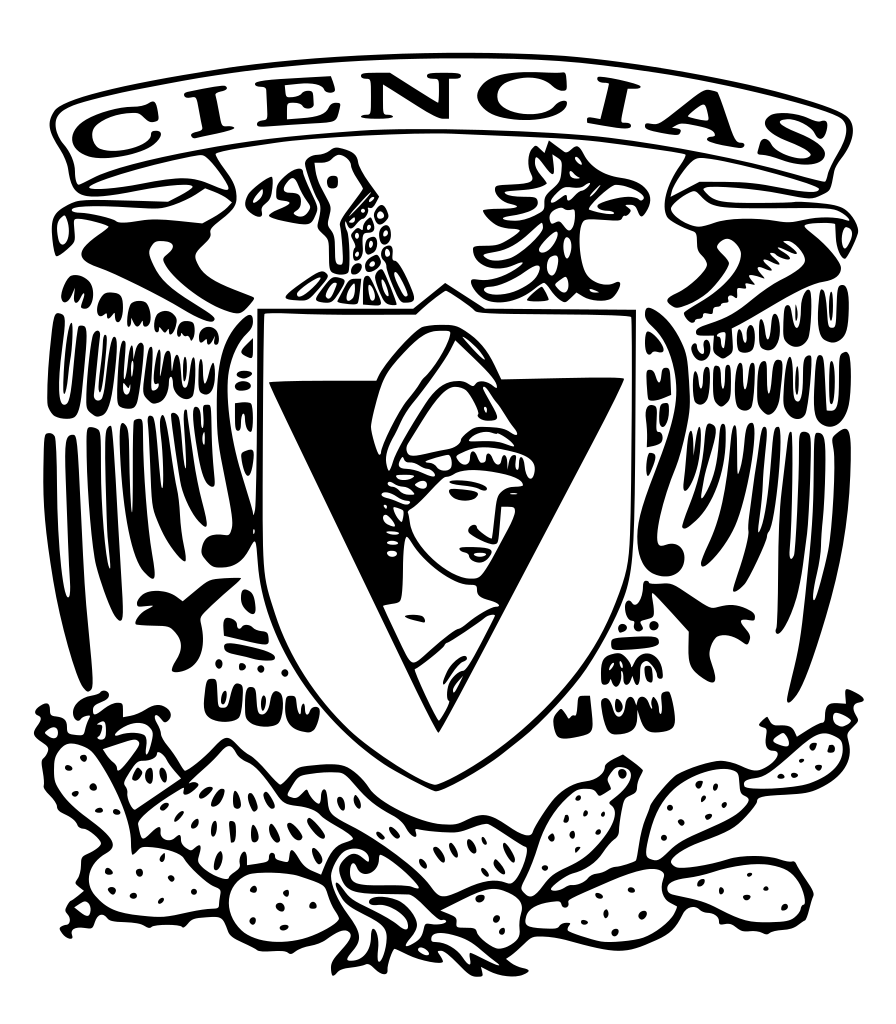
\includegraphics[scale=0.25]{3.png}
  \caption{Logo de la facultad de ciencias}
  \label{fig:fciencias}
\end{figure}

Podemos ver un ejemplo del logo de la facultad de ciencias en la
\emph{\textbf{figura}}~\ref{fig:fciencias}

\subsection{Hobbies}
Mis hobbies incluyen:
\begin{enumerate}
\item Escuchar música
\item Jugar videojuegos
\item Leer los libros ~\cite{torres, comunidad, retorno}
\end{enumerate}

\section{A profundidad}
Mucha gente se preguntará por qué decidí estudiar ciencias de la
computación. Este tema lo aboradré en las siguientes secciones
\subsection{Antecedentes}
Me gusta programar y me interesan las matemáticas.

\subsection{Las razones}
\begin{enumerate}
\item Me gusta programar
\item Me interesan las matemáticas
\end{enumerate}

\newpage
\section{Conocimientos}
\subsection{Leyes de los signos}
La \emph{\textbf{tabla}}~\ref{tab:signos} representa las leyes de los signos

\begin{table}[h]
  \centering
  \begin{tabular}{ c c c }
    Operando I & Operando II & Resultado\\
    \hline
    $+$ & $+$ & $+$\\
    $+$ & $-$ & $-$\\
    $-$ & $+$ & $-$\\
    $-$ & $-$ & $+$\\
  \end{tabular}
  \caption{Leyes de los signos}
  \label{tab:signos}
\end{table}

\subsection{Fórmulas importantes}
Algunas fórmulas importantes de mi vida son:
\begin{itemize}
\item $c^2 = a^2 + b^2$
\item $x = \frac{-b\pm\sqrt{b^2 - 4ac}}{2a}$
\end{itemize}

\section{Outro} 
\subsection{Agradecimientos}
Para el desarrollo de este libro, me gustaría hacer agradecimientos especiales
a los siguientes:
\begin{enumerate}
\item Mi familia
\item Mis maestros
\item Mis amigos
\item El lector
\end {enumerate}

\subsection{Palabras finales}
Este titulo tardó mucho tiempo en pensarse, desarrollarse, editarse e
inspeccionarse. Se ha llevado muchos tests de control para asegurarse de la
calidad del producto. Agradecemos su atención y ya.
